\documentclass[12pt, letterpaper]{article}

% ---------- Paquetes ----------
\usepackage[utf8]{inputenc}
\usepackage[T1]{fontenc}
\usepackage[spanish]{babel}
\usepackage{geometry}
\usepackage{setspace}
\usepackage{parskip}
\usepackage{graphicx}
\usepackage{float}
\usepackage{hyperref}
\usepackage{fancyhdr}
\usepackage{titlesec}
\usepackage{listings}
\usepackage{xcolor}
\usepackage{caption}
\usepackage{booktabs}
\usepackage{cite}
\usepackage{times}

% ---------- Geometría APA ----------
\geometry{
  letterpaper,
  left=2.54cm,
  right=2.54cm,
  top=2.54cm,
  bottom=2.54cm
}

% ---------- Interlineado doble ----------
\doublespacing

% ---------- Estilo de página ----------
\pagestyle{fancy}
\fancyhf{}
\rhead{\thepage}
\lhead{ACTIVIDAD \#1 -- METASPLOITABLE2}
\renewcommand{\headrulewidth}{0pt}

% ---------- Estilo de código ----------
\lstset{
  backgroundcolor=\color{gray!10},
  basicstyle=\ttfamily\footnotesize,
  breaklines=true,
  frame=single,
  rulecolor=\color{gray!40},
  keywordstyle=\color{blue},
  commentstyle=\color{green!50!black},
  stringstyle=\color{red!70!black},
  showstringspaces=false,
  tabsize=2,
  captionpos=b
}

% ---------- Secciones sin numeración automática estilo APA ----------
\titleformat{\section}{\normalfont\large\bfseries\centering}{}{0em}{}
\titleformat{\subsection}{\normalfont\normalsize\bfseries}{}{0em}{}
\titleformat{\subsubsection}{\normalfont\normalsize\bfseries\itshape}{}{0em}{}

% ==========================================================
\begin{document}

% ---------- Portada ----------
\begin{titlepage}
  \centering
  \vspace*{2cm}

  {\large Universidad Tecnológica de Pereira\\
  Facultad de Ingenierías\\
  Especialización en Tecnologías de la Información y las Comunicaciones\\[0.5em]
  Ciberseguridad}

  \vspace{3cm}

  {\LARGE \textbf{Actividad \#1 -- Metasploitable2:\\
  Explotación de Vulnerabilidades en Entornos Controlados}}

  \vspace{3cm}

  {\large Daniel Torosoto}

  \vfill

  {\large Pereira, Colombia\\
  Abril de 2026}
\end{titlepage}

% ---------- Tabla de contenidos ----------
\tableofcontents
\newpage

% ==========================================================
\section{Introducción}

La ciberseguridad ofensiva es una disciplina que permite a los profesionales de tecnología comprender y anticipar las técnicas utilizadas por actores maliciosos, con el fin de fortalecer la postura de seguridad de las organizaciones. En el marco de esta actividad académica, se exploran cinco vectores de ataque sobre la máquina virtual Metasploitable2, un entorno diseñado intencionalmente con vulnerabilidades conocidas para fines educativos.

Las tareas desarrolladas abarcan la explotación de backdoors mediante el framework Metasploit, ataques de inyección SQL y ejecución de comandos sobre la aplicación web DVWA (\textit{Damn Vulnerable Web Application}), ataques de fuerza bruta con Burp Suite e Hydra, y finalmente el cracking de contraseñas fuera de línea con John the Ripper.

Todas las pruebas se realizaron en un entorno aislado de red (modo Solo Anfitrión) sobre una Mac Mini M4, utilizando UTM como hipervisor para gestionar las máquinas virtuales Kali Linux (atacante) y Metasploitable2 (víctima).

% ==========================================================
\section{Configuración del Entorno}

\subsection{Descripción del entorno}

El entorno de laboratorio está compuesto por dos máquinas virtuales ejecutadas en UTM sobre una Mac Mini con procesador Apple M4. Ambas máquinas fueron configuradas con una única interfaz de red en modo Solo Anfitrión (\textit{Host-Only}), lo que garantiza el aislamiento total del tráfico respecto a redes externas.

\begin{table}[H]
  \centering
  \caption{\textit{Configuración de las máquinas virtuales}}
  \begin{tabular}{@{}lll@{}}
    \toprule
    \textbf{Máquina} & \textbf{Rol} & \textbf{Dirección IP} \\
    \midrule
    Kali Linux        & Atacante     & 192.168.128.3 \\
    Metasploitable2   & Víctima      & 192.168.128.2 \\
    \bottomrule
  \end{tabular}
\end{table}

\subsection{Herramientas del entorno}

\begin{itemize}
  \item \textbf{UTM}: Hipervisor para macOS/Apple Silicon que permite ejecutar máquinas virtuales x86\_64 mediante emulación QEMU.
  \item \textbf{Kali Linux}: Distribución GNU/Linux orientada a pruebas de penetración, que incluye de forma nativa herramientas como Metasploit, Nmap, sqlmap, Burp Suite, Hydra y John the Ripper.
  \item \textbf{Metasploitable2}: Distribución Ubuntu 8.04 configurada con servicios y aplicaciones deliberadamente vulnerables, diseñada para el entrenamiento en seguridad ofensiva.
\end{itemize}

\begin{figure}[H]
  \centering
  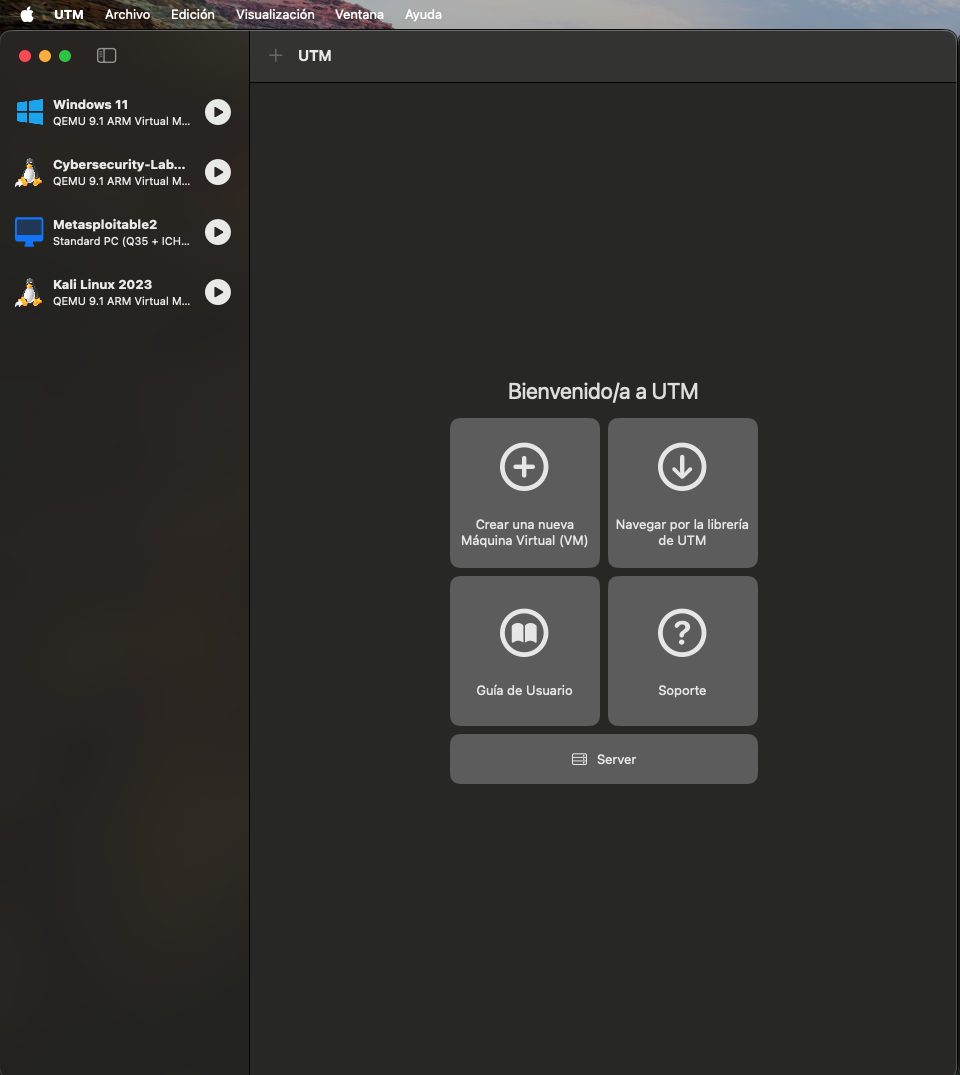
\includegraphics[width=0.85\textwidth]{../img/ambiente/utm.png}
  \caption{\textit{Vista del hipervisor UTM con las dos máquinas virtuales activas.}}
\end{figure}

\begin{figure}[H]
  \centering
  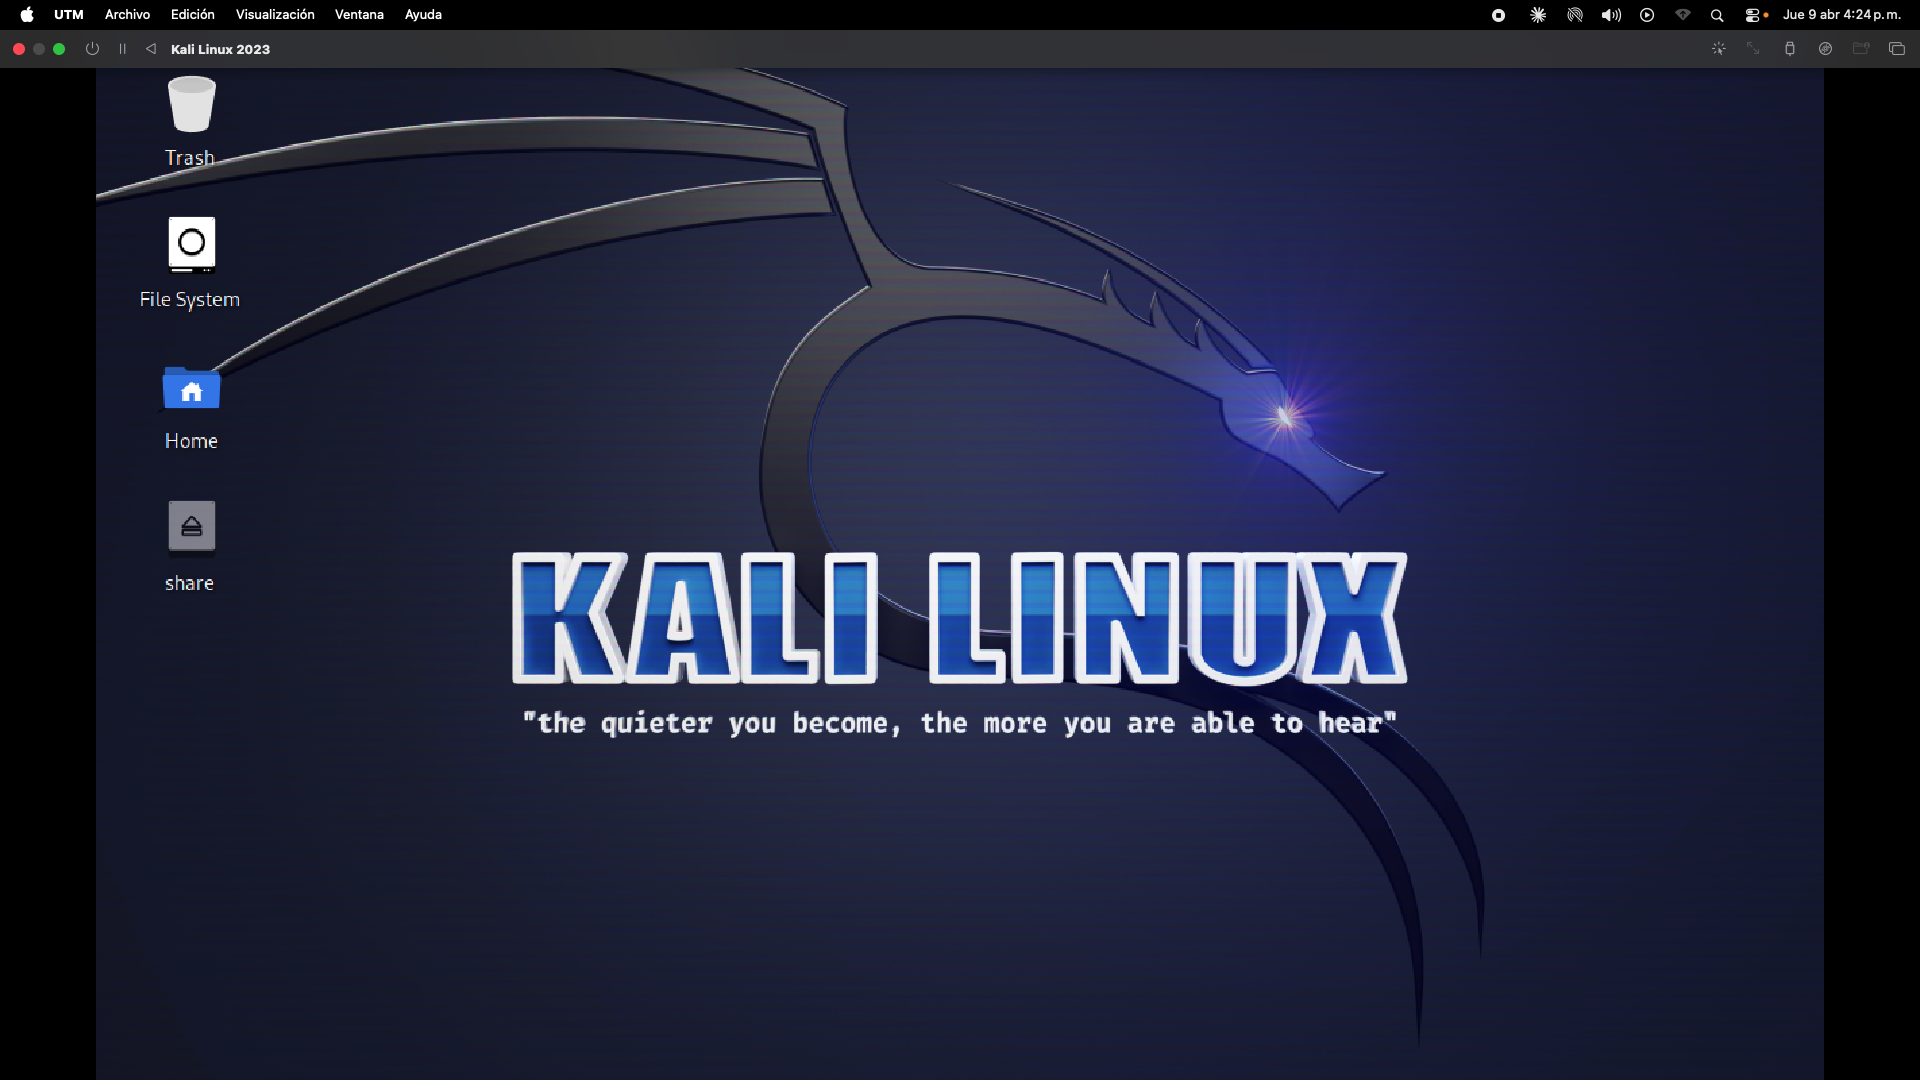
\includegraphics[width=0.85\textwidth]{../img/ambiente/kali.png}
  \caption{\textit{Máquina virtual Kali Linux (atacante) en ejecución.}}
\end{figure}

\begin{figure}[H]
  \centering
  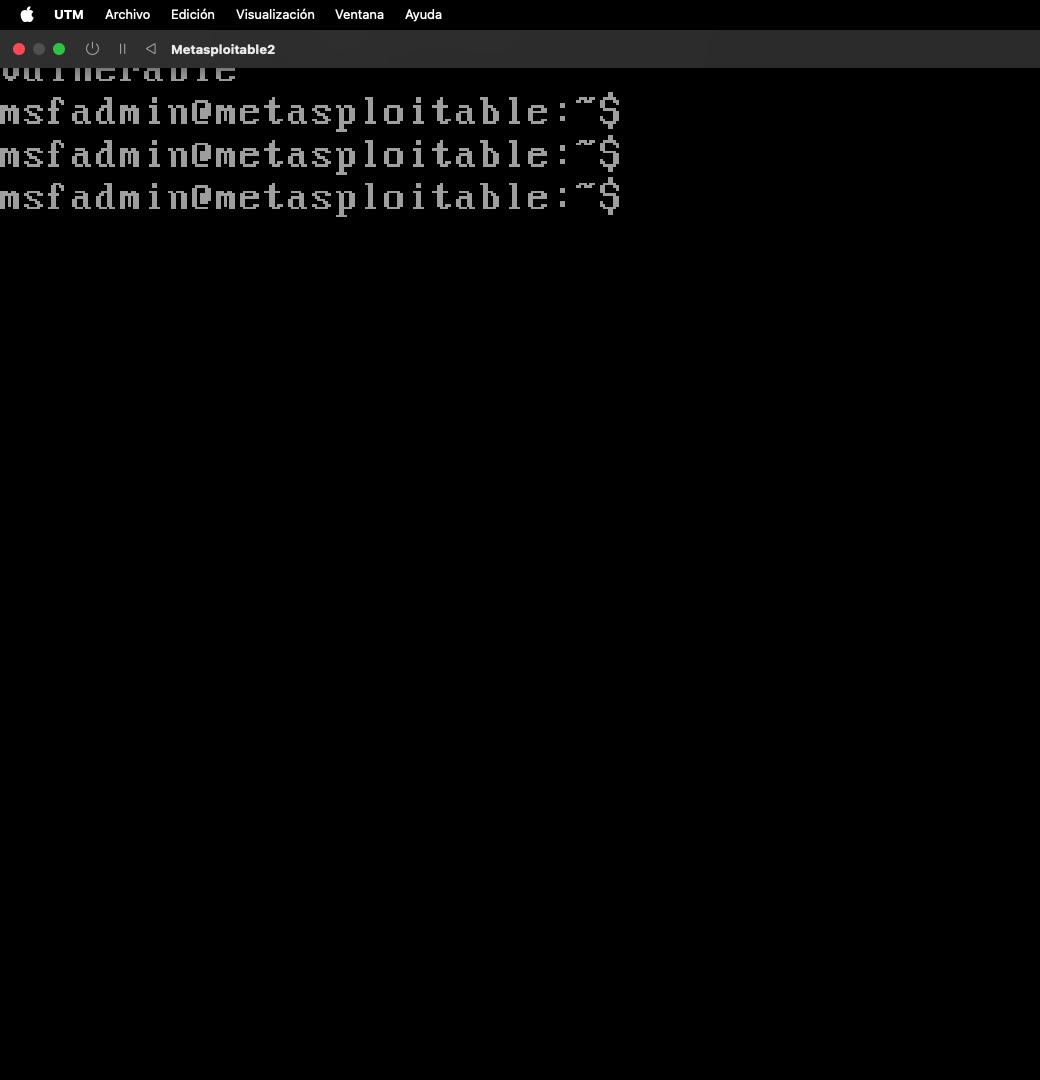
\includegraphics[width=0.85\textwidth]{../img/ambiente/metasploit2.png}
  \caption{\textit{Máquina virtual Metasploitable2 (víctima) en ejecución.}}
\end{figure}

% ==========================================================
\section{Tarea 1: Explotación de Backdoor en vsftpd 2.3.4}

\subsection{Descripción de la vulnerabilidad}

La vulnerabilidad CVE-2011-2523 afecta al demonio FTP \texttt{vsftpd} en su versión 2.3.4. Esta versión fue comprometida en su repositorio de distribución oficial en julio de 2011, cuando un atacante introdujo un backdoor en el código fuente. El mecanismo del backdoor consiste en que, al recibir una cadena de usuario que contiene los caracteres \texttt{:)} (carita feliz), el proceso abre una shell interactiva en el puerto TCP 6200 con privilegios de root, sin requerir autenticación alguna.

Esta vulnerabilidad es considerada crítica ya que otorga acceso completo al sistema con el máximo nivel de privilegios de forma trivial.

\subsection{Herramientas utilizadas}

\begin{itemize}
  \item \textbf{Nmap}: Escáner de red utilizado para descubrir hosts y servicios activos en la red, identificando la versión del servicio FTP vulnerable.
  \item \textbf{Metasploit Framework}: Framework de explotación de código abierto. Provee el módulo \texttt{exploit/unix/ftp/vsftpd\_234\_backdoor} que automatiza el proceso de activación y conexión al backdoor.
\end{itemize}

\subsection{Pasos realizados}

\subsubsection{Reconocimiento — Escaneo de red con Nmap}

El primer paso consistió en descubrir los hosts activos en la red y enumerar los servicios expuestos por Metasploitable2. Se ejecutó el siguiente comando desde Kali Linux:

\begin{lstlisting}[language=bash, caption={Escaneo de servicios con Nmap}]
nmap -sV 192.168.128.0/24
\end{lstlisting}

El resultado confirmó que Metasploitable2 (192.168.128.2) expone 22 servicios TCP, entre ellos el servicio FTP corriendo \texttt{vsftpd 2.3.4} en el puerto 21.

\begin{figure}[H]
  \centering
  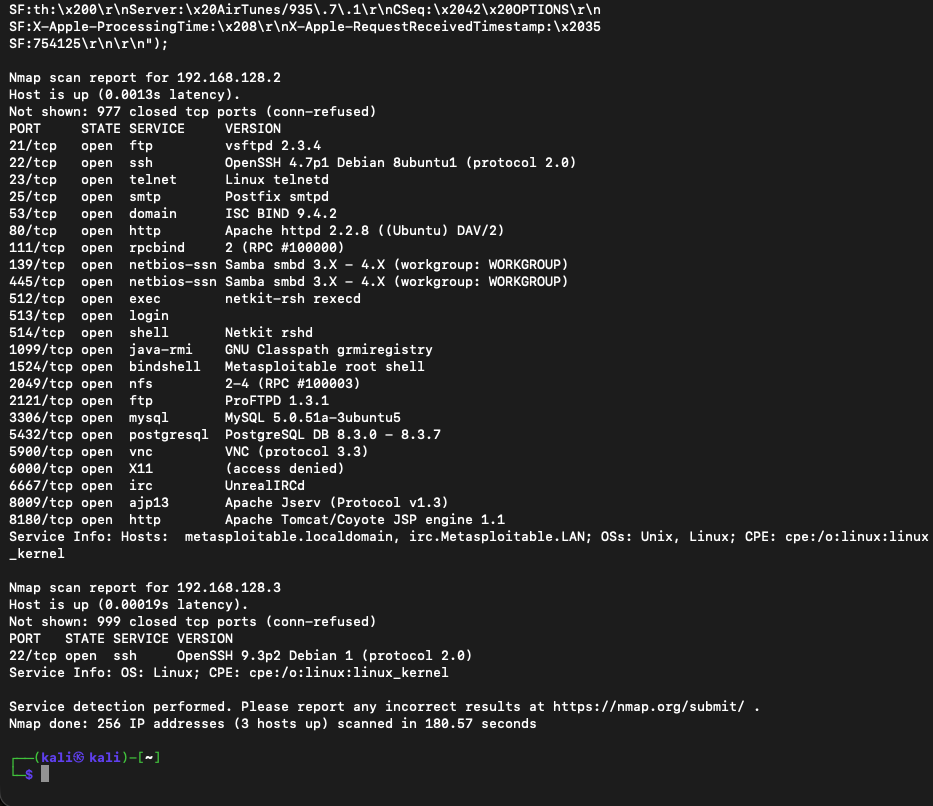
\includegraphics[width=0.92\textwidth]{../img/tarea1/t1_nmap_scan_kali.png}
  \caption{\textit{Resultado del escaneo Nmap mostrando los servicios activos en Metasploitable2, incluyendo vsftpd 2.3.4 en el puerto 21.}}
\end{figure}

\begin{figure}[H]
  \centering
  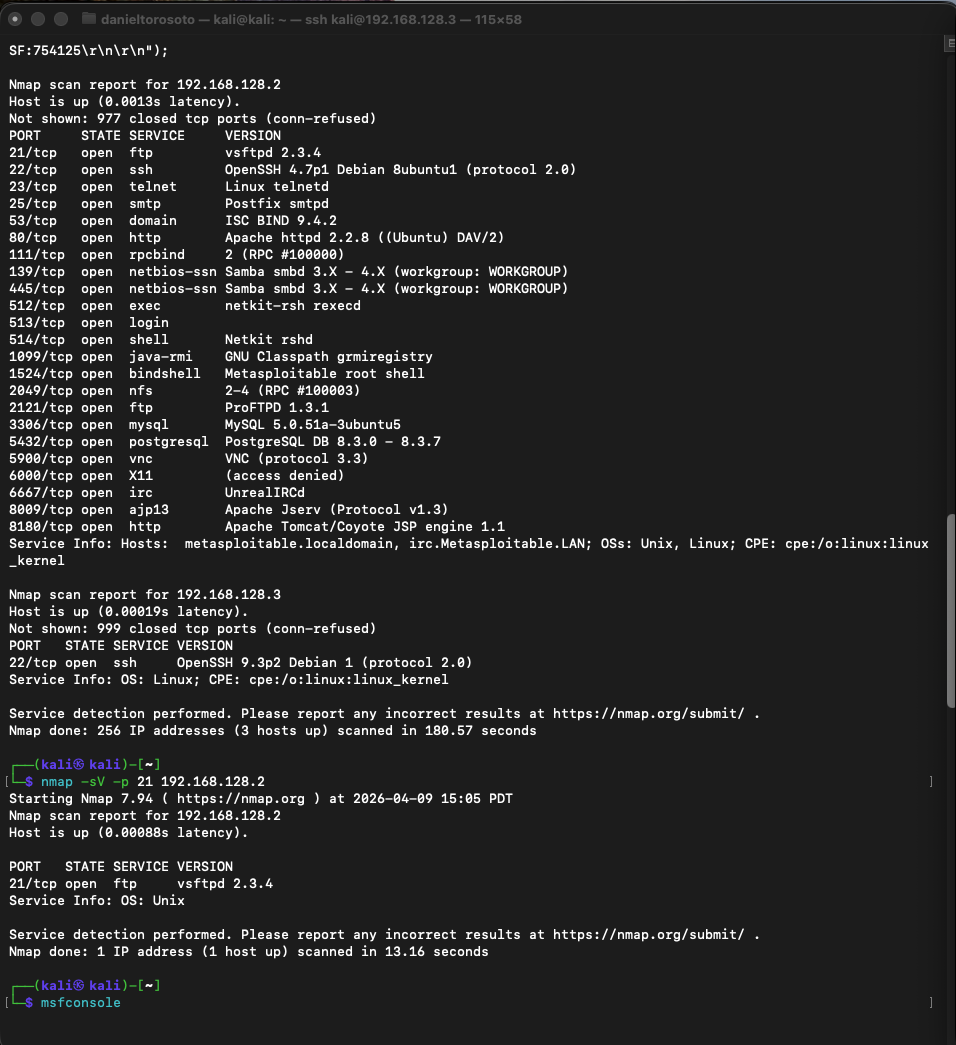
\includegraphics[width=0.92\textwidth]{../img/tarea1/t1_nmap_scan_port21_kali.png}
  \caption{\textit{Detalle del servicio FTP vsftpd 2.3.4 identificado en el puerto 21 de Metasploitable2.}}
\end{figure}

\subsubsection{Explotación con Metasploit Framework}

Se inició \texttt{msfconsole} y se cargó el módulo específico para la vulnerabilidad CVE-2011-2523:

\begin{lstlisting}[language=bash, caption={Configuración del módulo de explotación en Metasploit}]
use exploit/unix/ftp/vsftpd_234_backdoor
set RHOSTS 192.168.128.2
run
\end{lstlisting}

El módulo establece una conexión al servicio FTP de la víctima, envía las credenciales que contienen los caracteres \texttt{:)} para activar el backdoor, y luego se conecta al puerto 6200 donde la shell queda a la escucha. Al ejecutar el exploit, Metasploit confirmó la apertura de una sesión interactiva con el mensaje:

\begin{lstlisting}
[+] 192.168.128.2:21 - UID: uid=0(root) gid=0(root)
[*] Found shell.
[*] Command shell session 1 opened (192.168.128.3:44327 -> 192.168.128.2:6200)
\end{lstlisting}

\begin{figure}[H]
  \centering
  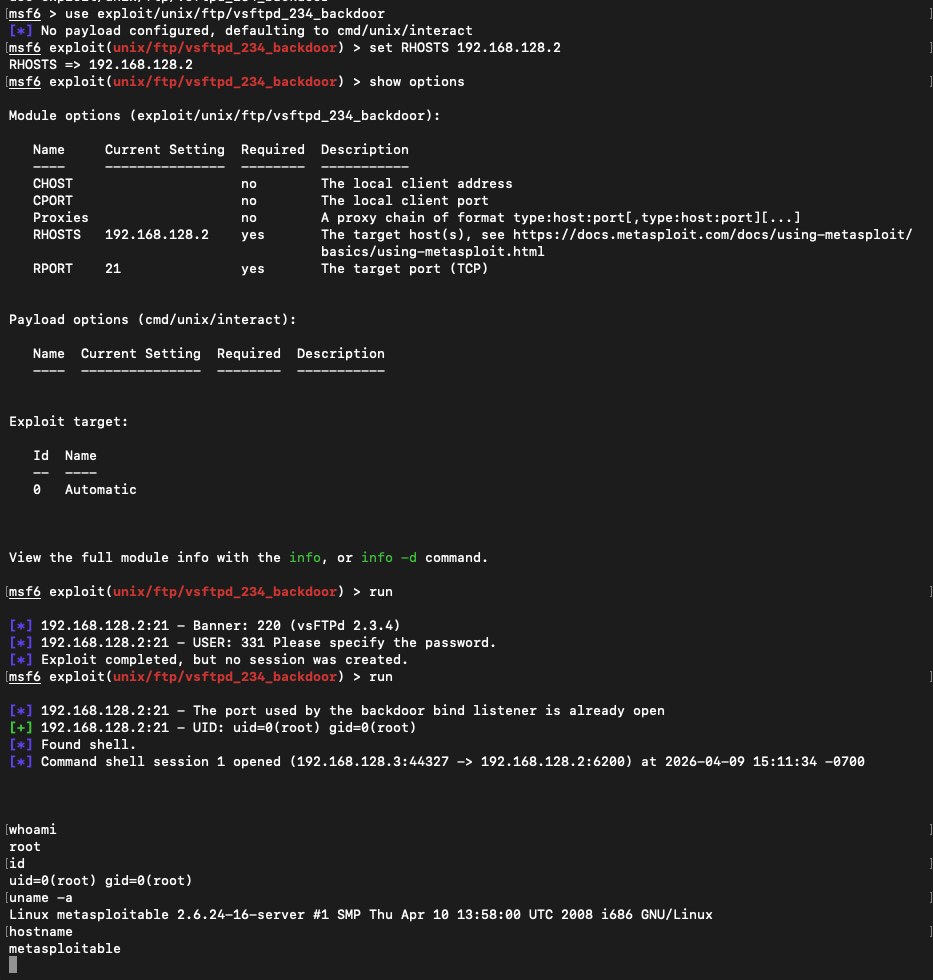
\includegraphics[width=0.92\textwidth]{../img/tarea1/t1_msfconsole_exploit_unix_ftp_vsftpd_234_backdoor.png}
  \caption{\textit{Ejecución del exploit en Metasploit Framework confirmando acceso root mediante backdoor en vsftpd 2.3.4.}}
\end{figure}

\subsection{Funcionamiento del ataque}

El ataque sigue el siguiente flujo:

\begin{enumerate}
  \item \textbf{Reconocimiento}: Nmap identifica el servicio vsftpd 2.3.4 en el puerto 21.
  \item \textbf{Activación del backdoor}: El módulo de Metasploit se conecta al puerto 21 y envía un nombre de usuario que termina con \texttt{:)} (por ejemplo, \texttt{user:)}). Esto activa el código malicioso insertado en el binario.
  \item \textbf{Apertura de la shell}: El proceso vsftpd comprometido abre una shell root en el puerto TCP 6200.
  \item \textbf{Conexión}: Metasploit se conecta automáticamente al puerto 6200 y establece una sesión interactiva con privilegios de root (\texttt{uid=0}).
\end{enumerate}

\subsection{Resultado}

Se obtuvo acceso total a Metasploitable2 con privilegios de superusuario (\texttt{uid=0(root) gid=0(root)}), demostrando el riesgo crítico que representa ejecutar software obtenido de fuentes comprometidas sin verificar su integridad.

% ==========================================================
\section{Tarea 2: SQL Injection en DVWA}

\subsection{Descripción de la vulnerabilidad}

% TODO: completar tras realizar la tarea

\subsection{Herramientas utilizadas}

% TODO: completar tras realizar la tarea

\subsection{Pasos realizados}

% TODO: completar tras realizar la tarea

\subsection{Funcionamiento del ataque}

% TODO: completar tras realizar la tarea

\subsection{Resultado}

% TODO: completar tras realizar la tarea

% ==========================================================
\section{Tarea 3: Command Execution en DVWA}

\subsection{Descripción de la vulnerabilidad}

% TODO: completar tras realizar la tarea

\subsection{Herramientas utilizadas}

% TODO: completar tras realizar la tarea

\subsection{Pasos realizados}

% TODO: completar tras realizar la tarea

\subsection{Funcionamiento del ataque}

% TODO: completar tras realizar la tarea

\subsection{Resultado}

% TODO: completar tras realizar la tarea

% ==========================================================
\section{Tarea 4: Fuerza Bruta a DVWA}

\subsection{Descripción de la vulnerabilidad}

% TODO: completar tras realizar la tarea

\subsection{Herramientas utilizadas}

% TODO: completar tras realizar la tarea

\subsection{Pasos realizados}

% TODO: completar tras realizar la tarea

\subsection{Funcionamiento del ataque}

% TODO: completar tras realizar la tarea

\subsection{Resultado}

% TODO: completar tras realizar la tarea

% ==========================================================
\section{Tarea 5: Cracking de Contraseñas con John the Ripper}

\subsection{Descripción de la vulnerabilidad}

% TODO: completar tras realizar la tarea

\subsection{Herramientas utilizadas}

% TODO: completar tras realizar la tarea

\subsection{Pasos realizados}

% TODO: completar tras realizar la tarea

\subsection{Funcionamiento del ataque}

% TODO: completar tras realizar la tarea

\subsection{Resultado}

% TODO: completar tras realizar la tarea

% ==========================================================
\section{Conclusiones}

% TODO: completar al finalizar todas las tareas

% ==========================================================
\section{Referencias}

\begin{itemize}
  \item Kennedy, D., O'Gorman, J., Kearns, D., \& Aharoni, M. (2011). \textit{Metasploit: The Penetration Tester's Guide}. No Starch Press.
  \item Offensive Security. (2024). \textit{Metasploit Unleashed}. \url{https://www.offsec.com/metasploit-unleashed/}
  \item National Vulnerability Database. (2011). \textit{CVE-2011-2523}. \url{https://nvd.nist.gov/vuln/detail/CVE-2011-2523}
  \item OWASP. (2021). \textit{OWASP Top Ten}. \url{https://owasp.org/www-project-top-ten/}
  \item Rapid7. (2024). \textit{Metasploit Framework Documentation}. \url{https://docs.metasploit.com/}
\end{itemize}

\end{document}
